\documentclass[conference]{IEEEtran}
\IEEEoverridecommandlockouts
% The preceding line is only needed to identify funding in the first footnote. If that is unneeded, please comment it out.
\usepackage{cite}
\usepackage{amsmath,amssymb,amsfonts}
\usepackage{algorithmic}
\usepackage{graphicx}
\usepackage{textcomp}
\usepackage{xcolor}
\usepackage{url}
\def\BibTeX{{\rm B\kern-.05em{\sc i\kern-.025em b}\kern-.08em
    T\kern-.1667em\lower.7ex\hbox{E}\kern-.125emX}}

\begin{document}

\title{Codec Development for Converting Digital Music Files into DNA Sequences Based on Automatic Notation Transcription and Tokenization}

\author{\IEEEauthorblockN{Robertus Hudi}
\IEEEauthorblockA{\textit{Faculty of Artificial Intelligence and Data Science} \\
\textit{Universitas Pelita Harapan}\\
Tangerang, Indonesia \\
robertus.hudi@uph.edu}
\and
\IEEEauthorblockN{Teofilus Satria Rada Insani}
\IEEEauthorblockA{\textit{Faculty of Artificial Intelligence and Data Science} \\
\textit{Universitas Pelita Harapan}\\
Tangerang, Indonesia \\
01082230015@student.uph.edu}
}

\maketitle

\begin{abstract}
DNA data storage is priced per synthesised nucleotide, so the number of bases written determines its cost. Music recordings are usually stored by mapping the bytes of the audio file directly to nucleotides, which gains nothing from musical structure because compressed audio is already close to its entropy. This paper presents a codec that changes the representation first: audio is transcribed into notes, quantised to a rhythmic grid, encoded as fixed-width feature tokens with repeated phrases replaced by back-references, and mapped to oligonucleotides by a Reed--Solomon outer code and a rotating inner code that enforces biochemical constraints. The codec was evaluated on 82 piano and guitar stems from the Slakh dataset (4.6 h of audio, 67,964 notes), whose format, signal and musical content are characterised quantitatively, with the transcription threshold calibrated on a separate development split. Read-back was lossless for every sample, and all 4,770 oligonucleotides met the GC-content and homopolymer constraints. The token scheme required 85.0\% fewer bases than encoding the transcribed MIDI file, and repeat detection alone removed 43.2\%. The note-level F-measure averaged 0.748; the DNA layer was lossless, while reconstruction error was dominated by transcription, with quantisation having no significant effect on the whole-system F-measure. Two further effects are quantified: Reed--Solomon codeword granularity masks repeat detection on short payloads, and transcription errors remove a quarter of the repetition present in the reference notation.
\end{abstract}

\begin{IEEEkeywords}
DNA data storage, automatic music transcription, constrained coding, Reed--Solomon code, symbolic music compression
\end{IEEEkeywords}

\section{Introduction}

Digital archives must be migrated long before their media wear out. A hard disk is typically retired after three to five years, and although LTO tape is rated for thirty, each drive generation reads only about two generations back, so tape archives are rewritten every five to ten years regardless of the condition of the cartridges \cite{dong}, \cite{lto}. Every migration costs energy and labour and risks loss. Music collections of cultural value are particularly exposed, because their carriers and their file formats both become obsolete.

DNA avoids both problems \cite{shomorony}. Erlich and Zielinski retrieved data without error from a library at 215 petabytes per gram \cite{erlich}, and accelerated-ageing experiments on silica-encapsulated DNA indicate information lifetimes of about two thousand years under central-European storage conditions and beyond a million years at $-18^\circ$C \cite{grass}. Neither property requires a power supply, and because sequencing is sustained by biology and medicine, reading the medium does not depend on a storage product line. Music has already been archived this way: the Montreux Jazz Festival recordings of \textit{Smoke on the Water} and \textit{Tutu} were encoded in DNA and read back exactly \cite{dufaux}, and a melody has been stored by enzymatic synthesis \cite{lee}.

The obstacle is cost, which is charged per nucleotide. Array-based synthesis costs on the order of $10^{-4}$ USD per base, whereas tape archiving is seven to eight orders of magnitude cheaper per terabyte \cite{yu}, so reducing the number of bases is the most direct lever on feasibility. Mapping the bytes of an MP3 file to DNA provides no such reduction, because the final stage of MP3 encoding is Huffman coding and leaves the bytes close to their entropy. Music is nevertheless highly structured: its pitches, rhythms and repeated motifs can be expressed far more compactly in symbolic form \cite{benetos}. Repetition in particular can only be exploited symbolically, since two renditions of the same phrase rarely produce identical audio samples.

This paper presents a codec that stores a recording in DNA through such a representation. Its contributions are: (i) an end-to-end pipeline that connects automatic music transcription to constraint-compliant DNA encoding through a compact token scheme with token-level repeat detection; (ii) an evaluation on a quantitatively characterised corpus of 82 held-out stems that attributes loss to individual modules; and (iii) a quantification of two interactions that limit the achievable saving, namely the masking of repeat detection by Reed--Solomon codeword granularity and the loss of repetition caused by transcription errors.

\section{Related Work}

\subsection{Coding for DNA Data Storage}

Church et al. \cite{church} and Goldman et al. \cite{goldman} demonstrated megabit-scale storage in synthetic DNA. Goldman et al. introduced the rotating code, in which each base-3 symbol selects one of the three nucleotides that differ from the preceding base, so that homopolymers cannot occur, at 1.58 bits per base. Grass et al. \cite{grass} added a Reed--Solomon outer code, establishing the division into a byte-level outer code across oligonucleotides and a base-level inner code within each one that is also used here. Later work raised density or robustness. Fountain codes reached a net 1.57 bits per base \cite{erlich}, with recovery methods since refined \cite{schwarz}, and per-file primer pairs provided random access at the scale of 200 MB \cite{organick}. Constraints on GC content, homopolymer length and forbidden motifs are now met by construction through chaos-game code words \cite{lochel}, two-rule transcoding \cite{ping}, adaptive thresholds \cite{cao} and arithmetic coding \cite{welzel}, while HEDGES also corrects insertions and deletions \cite{press} and combinatorial shortmer encoding raises density further \cite{preuss}. Surveys of the field \cite{dong}, \cite{shomorony}, \cite{xu} and of synthesis \cite{yu} stress that synthesis yield falls with strand length and that every strand must carry an address and primers, so short oligonucleotides and tight overhead accounting matter. All of these schemes are content-agnostic: they encode whatever bytes they are given.

\subsection{Music, Transcription and DNA}

Automatic music transcription estimates the pitch, onset and offset of every note in a recording. Polyphonic material remains difficult, and errors take three forms: missed notes, spurious notes that are often harmonics of real ones, and notes with displaced onsets or offsets \cite{benetos}. The basic-pitch model \cite{bittner} is instrument-agnostic and light enough for inference on a CPU. Existing work on music in DNA starts from symbolic input: Antkowiak et al. stored a MusicXML score \cite{antkowiak}, Lee et al. encoded the note numbers, octaves and durations of a melody \cite{lee}, and Kiryanova et al. encoded melodies over seven octaves more compactly than Huffman coding \cite{kiryanova}. None of these begins from a recording, and none exploits repetition, which LZ77 \cite{ziv} removes by replacing a repeated sequence with a reference to an earlier occurrence. Combining transcription, symbolic compression and constrained DNA coding, and measuring what each stage costs and saves, is the gap this paper addresses.

\section{Proposed Codec}

\begin{figure*}[t]
\centering
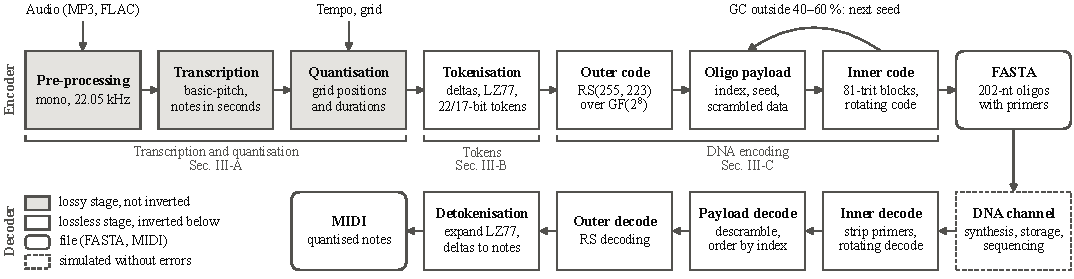
\includegraphics[width=\textwidth]{fig1.pdf}
\caption{Architecture of the codec. Each lossless encoder stage is inverted by the decoder stage beneath it; the shaded stages are lossy and have no inverse. Brackets mark the subsections of Section~III that describe each group.}
\label{fig:architecture}
\end{figure*}

Fig.~\ref{fig:architecture} shows the codec. The encoder pre-processes and transcribes the audio, quantises the notes, converts them to tokens and encodes the resulting bytes into oligonucleotides written in FASTA format. The decoder inverts only the lossless stages: it recovers the quantised notes and writes them as MIDI, since the timing detail removed by transcription and quantisation cannot be restored. Tempo and grid travel in the header, so decoding needs no side information.

\subsection{Transcription and Quantisation}

The audio is downmixed to mono, resampled to 22.05 kHz and transcribed with basic-pitch \cite{bittner} using an onset threshold of 0.7, chosen as described in Section~\ref{subsec:calibration}, a frame threshold of 0.3 and a minimum note length of 60 ms; the library default of 127.7 ms would discard every sixteenth note above 117 BPM. The notes are then quantised to a grid of 1/4, 1/8, 1/16 or 1/24 of a whole note at a tempo stored in the header, both of which are chosen per piece (Section~\ref{subsec:dataset}). Each note becomes a pitch, an onset position and a duration in grid units, and notes with the same pitch and position are merged.

\subsection{Token Scheme}

Fig.~\ref{fig:layout}(a) shows the token formats. A 32-bit header stores the schema version, the tempo (40--295 BPM), the grid code and the token count. Each note is a 22-bit token holding a type bit, the pitch (7 bits), the onset delta from the previous note (8 bits, up to 255 grid units) and the duration (6 bits, 1--64 units, longer notes being clamped). Storing deltas rather than absolute positions makes identical phrases produce identical token sequences wherever they occur, which repeat detection requires. An LZ77-style search \cite{ziv} then replaces the longest repeated run of 2--65 tokens within the preceding 1,024 by a 17-bit reference token holding a type bit, the distance and the length. Because a reference replaces at least 44 bits, every match saves space. Fig.~\ref{fig:layout}(c) shows the effect on a four-note motif played twice: the absolute onsets of the two occurrences differ, but their deltas are identical, so the second occurrence becomes a single reference and the token stream shrinks from 176 to 105 bits.

\begin{figure}[htbp]
\centering
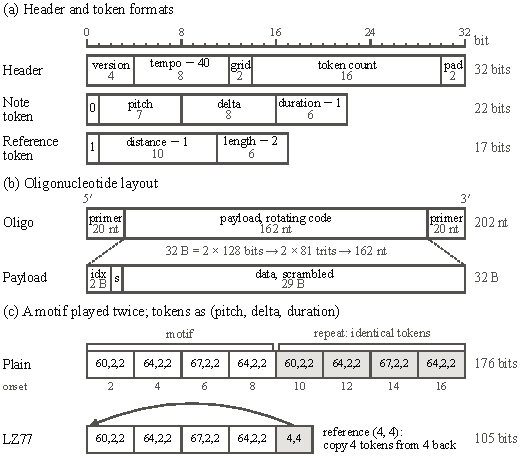
\includegraphics[width=\columnwidth]{fig2.pdf}
\caption{(a) Header and token formats; the leading bit is 0 for a note and 1 for a reference, and each field is stored with an offset so that its full range is usable. (b) Oligonucleotide layout; the 32-byte payload carries a 2-byte index (idx) and a 1-byte seed (s) in the clear, followed by 29 scrambled data bytes, and is converted as two 128-bit blocks of 81 trits into 162 nt. (c) Tokens of a four-note motif played twice, with absolute onsets in grid units beneath; the repeat (shaded) has the same deltas and is replaced by one reference token (distance 4, length 4).}
\label{fig:layout}
\end{figure}

\subsection{DNA Encoding}

The token bytes are protected by an RS(255,\,223) code over $\mathrm{GF}(2^8)$ \cite{reed}, which corrects 16 symbol errors per codeword, and divided into oligonucleotides that each carry a 2-byte index, a 1-byte scrambling seed and 29 data bytes. The data bytes are XORed with a keystream derived from SHA-256 so that GC content concentrates near 50\%. The resulting 32-byte payload is converted, as two 128-bit blocks of 81 trits each, into 162 bases with the rotating code \cite{goldman}, the first base being rotated against the last base of the forward primer. Each oligonucleotide is 202 nt long (Fig.~\ref{fig:layout}(b)): a 20-nt forward primer, 162 nt of payload and a 20-nt reverse primer. An oligonucleotide whose GC content falls outside 40--60\% is re-scrambled with the next seed. The layout bounds the effective density at
\begin{equation}
\rho_{\max} = \frac{128}{81}\cdot\frac{162}{202}\cdot\frac{29}{32}\cdot\frac{223}{255} \approx 1.004\ \text{bits per base}.
\label{eq:ceiling}
\end{equation}

\section{Experimental Setup}

\subsection{Dataset}
\label{subsec:dataset}

Slakh \cite{slakh} renders MIDI files from the Lakh collection with sample-based virtual instruments, so every audio stem comes with an exactly aligned reference transcription. We drew 151 single-stem tracks and adapted them to the token scheme in three steps. First, 56 tracks whose MIDI contains a tempo map were excluded, because the header holds a single tempo. Second, the tempo and grid of each remaining piece were chosen among the notated tempo, half and double that tempo and the four grid resolutions, by minimising the RMS deviation of the reference onsets from the grid. Lakh files are often notated at half or double their felt tempo and some pieces use triplets, and the best fit differed from the notated tempo on a sixteenth-note grid for 50 of the 95 pieces; five pieces still lay more than a quarter of a grid unit off after fitting and were excluded, together with one piece of fewer than 32 notes. Third, 15 stems that rest for longer than the 255 grid units an 8-bit delta can span were cut at the rest, on a grid boundary. This yielded 100 samples from 89 tracks, which were split by track into 18 development and 82 test samples, stratified by instrument.

Table~\ref{tab:dataset} characterises the 82 test samples (71 tracks, 4.6 h, 67,964 notes). Their format is uniform, but their content is not. The stems use 15 General MIDI programs rendered with 26 distinct instrument patches, ranging from grand and bright pianos to harpsichord and clavinet and from nylon- and steel-string acoustic guitars to distorted electric guitars. The material is strongly polyphonic: on average 2.5 notes sound together, and 62\% of the notes start within 30 ms of another. On average the guitar stems are longer than the piano stems, contain fewer chords and span a narrower pitch range, and they vary more in level and spectrum. Tempi range from 40 to 226 BPM; 64 samples use a sixteenth-note grid, 12 a sextuplet grid and six coarser grids. After fitting, reference onsets deviate from the grid by only 0.05 units on average, so the pieces are metrically regular. The reference notation is highly repetitive, with repeat detection removing 62.1\% of its tokens. For the stratified analyses, samples were labelled by corpus terciles, with boundaries at 173 and 238 s for duration, 3.2 and 4.7 notes/s for density and 52.4\% and 78.6\% for repetition.

\begin{table}[htbp]
\caption{Characteristics of the Test Split}
\label{tab:dataset}
\centering
\footnotesize
\setlength{\tabcolsep}{3pt}
\begin{tabular}{lrrr}
\hline
 & \textbf{Piano} & \textbf{Guitar} & \textbf{All} \\
\hline
Samples & 48 & 34 & 82 \\
GM programs / patches & 8 / 15 & 7 / 11 & 15 / 26 \\
\multicolumn{4}{l}{\textit{Format} (every sample: FLAC, 16-bit PCM, 44.1 kHz, mono)} \\
Bitrate (kbit/s) & 150 $\pm$ 41 & 153 $\pm$ 82 & 151 $\pm$ 61 \\
\multicolumn{4}{l}{\textit{Signal}} \\
Duration (s) & 190 $\pm$ 108 & 224 $\pm$ 70 & 204 $\pm$ 95 \\
Loudness (LUFS) & $-24.5 \pm 3.6$ & $-22.4 \pm 6.8$ & $-23.6 \pm 5.2$ \\
Sounding time (\%) & 85 $\pm$ 14 & 78 $\pm$ 22 & 82 $\pm$ 18 \\
Peak level (dBFS) & $-9.6 \pm 2.8$ & $-13.3 \pm 4.1$ & $-11.2 \pm 3.8$ \\
Spectral centroid (Hz) & 795 $\pm$ 274 & 851 $\pm$ 486 & 818 $\pm$ 375 \\
\multicolumn{4}{l}{\textit{Musical content (reference notation)}} \\
Notes per sample & 779 $\pm$ 585 & 899 $\pm$ 664 & 829 $\pm$ 618 \\
Density (notes/s) & 4.18 $\pm$ 2.13 & 4.48 $\pm$ 3.07 & 4.31 $\pm$ 2.55 \\
Mean polyphony & 2.58 $\pm$ 0.97 & 2.35 $\pm$ 1.00 & 2.48 $\pm$ 0.99 \\
Notes in chords (\%) & 68 $\pm$ 30 & 55 $\pm$ 36 & 62 $\pm$ 33 \\
Pitch, P5--P95 (MIDI) & 41--79 & 42--71 & 42--76 \\
Note length (beats) & 0.51 $\pm$ 0.38 & 0.72 $\pm$ 0.91 & 0.60 $\pm$ 0.66 \\
Velocity & 91 $\pm$ 17 & 90 $\pm$ 19 & 91 $\pm$ 18 \\
Tempo (BPM) & 91 $\pm$ 34 & 104 $\pm$ 43 & 96 $\pm$ 38 \\
Grid deviation (units) & 0.05 $\pm$ 0.05 & 0.05 $\pm$ 0.05 & 0.05 $\pm$ 0.05 \\
Repetition (\%) & 63.0 $\pm$ 22.3 & 60.8 $\pm$ 27.9 & 62.1 $\pm$ 24.6 \\
\hline
\multicolumn{4}{l}{Mean $\pm$ SD over samples. Loudness from Slakh metadata;} \\
\multicolumn{4}{l}{note length is a per-sample median; repetition is the} \\
\multicolumn{4}{l}{share of reference tokens removed by LZ77.} \\
\end{tabular}
\end{table}

\subsection{Baselines and Metrics}
\label{subsec:metrics}

Two references are measured with the same DNA scheme, so that differences in base count reflect the payload alone. B2, the MIDI file produced by transcription before quantisation and tokenisation, is encoded through the codec. B1, the bytes of the audio file, is counted rather than encoded: its base count is computed analytically from the same RS(255,\,223) code and per-oligonucleotide overhead, without building the oligonucleotides. Where the audio would exceed the 16-bit oligonucleotide address space, B1 is therefore an analytical size baseline rather than a supported round-trip encoding. The saving against a reference with $N_{\mathrm{ref}}$ bases is $1 - N/N_{\mathrm{ref}}$. The saving against B2 isolates the token scheme, since both paths share the same transcription. Effective density is the number of payload bits per synthesised base and is bounded by (\ref{eq:ceiling}). Note-level accuracy is measured with mir\_eval \cite{raffel} at an onset tolerance of 50 ms and a pitch tolerance of 50 cents, and additionally with an offset tolerance equal to the larger of 50 ms and 20\% of the note duration. To attribute loss, transcription is scored against the reference, the decoded notes against the transcription, and the whole system against the reference, while codec correctness is checked by comparing SHA-256 digests of the token stream before encoding and after decoding.

\subsection{Calibration and Implementation}
\label{subsec:calibration}

The onset threshold was chosen on the development split alone. As it increased from 0.30 to 0.80, precision rose and recall fell monotonically, and the mean F-measure rose from 0.555 to 0.683 at 0.70 before falling to 0.676 at 0.80; at 0.30 the model produced 2.38 notes per reference note. The best value, 0.70, was used for the test split. Thresholds from 0.50 to 0.80 all lay within one standard error of it, the between-piece standard deviation being 0.24, so the choice is only weakly determined by the data. The codec is implemented in Python 3.11.3 with basic-pitch 0.4.0 on a CPU runtime of TensorFlow 2.15, reedsolo 1.7.0, Biopython 1.87, music21 10.5.0, mir\_eval 0.8.2 and pretty\_midi 0.2.11, and is verified by 198 unit tests. The primers are \texttt{ACGTAGCTAGCATGCATCGA} (forward) and \texttt{TGCATCGATCGTACGATGCA} (reverse), both written 5$'$ to 3$'$. Transcription runs about 91 times faster than real time (a real-time factor of about 0.011), and encoding and decoding the whole test split took 14 min. The source code, codec configuration, corpus manifests and evaluation scripts are available at \url{https://github.com/pejuangvscode/MP3-to-DNA}.

\section{Results and Discussion}

\subsection{Correctness and Constraint Compliance}

All 82 samples decoded to token streams identical to those encoded, and encoding was deterministic. All 4,770 oligonucleotides met the constraints without re-scrambling: GC content ranged from 0.431 to 0.584 per oligonucleotide, with per-sample means of $0.504 \pm 0.004$, and the longest homopolymer was two bases in 81 samples and one in the remaining one. Runs of two occur only at the junction with the fixed reverse primer, whose first base the final, data-dependent payload base matches with a probability of about one in four, so with dozens of oligonucleotides per sample such a junction almost always appears; the bound of three is never reached. The DNA layer therefore introduces no loss, and all reconstruction error originates in transcription and quantisation.

\subsection{Base Efficiency}

Table~\ref{tab:results} lists base counts and accuracy by instrument. The codec needed 963,540 bases for the whole test split, 85.0\% fewer than the transcribed MIDI files (B2) and 99.96\% fewer than the audio files (B1). The saving against B1 mostly reflects the change from audio to notation, and it is inflated because Slakh distributes lossless FLAC rather than MP3. The saving against B2, which holds the transcription fixed, is the contribution of the token scheme, and it is almost the same for piano (85.2\%) and guitar (84.9\%). The effective density averaged 0.839 bits per base and reached 1.000, or 99.5\% of $\rho_{\max}$, in the best sample. The direct baseline also revealed a limit of the addressing scheme: the 2-byte index allows 65,536 oligonucleotides, about 1.6 MiB, which B1 would exceed for 67 of the 82 samples, the shortest being 64 s long. For those samples the B1 count is analytical only and could not be stored as a single archive under the present index, whereas the largest token encoding needed 229 oligonucleotides.

\begin{table}[htbp]
\caption{Efficiency and Accuracy on the Test Split}
\label{tab:results}
\centering
\footnotesize
\setlength{\tabcolsep}{3pt}
\begin{tabular}{lrrr}
\hline
 & \textbf{Piano} & \textbf{Guitar} & \textbf{All} \\
\hline
\multicolumn{4}{l}{\textit{Bases synthesised (total)}} \\
Proposed codec & 527,018 & 436,522 & 963,540 \\
B2: MIDI & 3,551,968 & 2,884,156 & 6,436,124 \\
B1: audio ($\times 10^{6}$)$^{*}$ & 1,368 & 1,144 & 2,512 \\
Saving vs.\ B2 (\%) & 85.2 & 84.9 & 85.0 \\
\multicolumn{4}{l}{\textit{Per sample}} \\
Saving by LZ77 (\%) & 44.4 $\pm$ 26.2 & 41.5 $\pm$ 24.1 & 43.2 $\pm$ 25.2 \\
Density (bit/base) & 0.816 $\pm$ 0.170 & 0.872 $\pm$ 0.133 & 0.839 $\pm$ 0.157 \\
Precision & 0.732 $\pm$ 0.138 & 0.635 $\pm$ 0.179 & 0.692 $\pm$ 0.162 \\
Recall & 0.918 $\pm$ 0.092 & 0.736 $\pm$ 0.227 & 0.842 $\pm$ 0.184 \\
F-measure & 0.806 $\pm$ 0.099 & 0.666 $\pm$ 0.177 & 0.748 $\pm$ 0.152 \\
F with offset & 0.286 $\pm$ 0.172 & 0.300 $\pm$ 0.160 & 0.292 $\pm$ 0.167 \\
F, transcription & 0.811 $\pm$ 0.104 & 0.689 $\pm$ 0.164 & 0.761 $\pm$ 0.145 \\
\hline
\multicolumn{4}{l}{$^{*}$Counted analytically, not encoded (Section~\ref{subsec:metrics}).} \\
\end{tabular}
\end{table}

\subsection{Repeat Detection and Codeword Granularity}

Repeat detection reduced the base count of a sample by $43.2 \pm 25.2$\%, and by 48.7\% over the whole split, and the reduction closely tracked the repetitiveness of the reference notation (Spearman $\rho = 0.87$): 16.2\%, 45.3\% and 68.0\% in the low, medium and high repetition terciles. It did not reduce the base count at all in ten samples. In five of them the token stream shrank by 20--41\%, but the payload remained within the same number of RS(255,\,223) codewords. Every codeword is padded to 223 data bytes and synthesised in full, so the base count cannot change until a codeword boundary is crossed. The other five samples contained little repetition to remove (2--15\% of tokens).

Fig.~\ref{fig:results}(a) shows the consequence for density. Samples that fit in a single codeword average 0.610 bits per base, and density rises with payload size (Spearman $\rho = 0.83$) to 0.791, 0.938 and 0.965 for samples of 10--49, 50--99 and 100 or more oligonucleotides. Just above a codeword boundary the density drops sharply, since a nearly empty codeword is synthesised in full; the effect is largest at the first boundary and fades as codewords accumulate. Efficiency measured on short excerpts therefore understates the scheme, and a compression stage should be reported at the token level as well as the base level. A shortened Reed--Solomon code, whose padding is not synthesised, would remove the effect.

\begin{figure}[htbp]
\centering
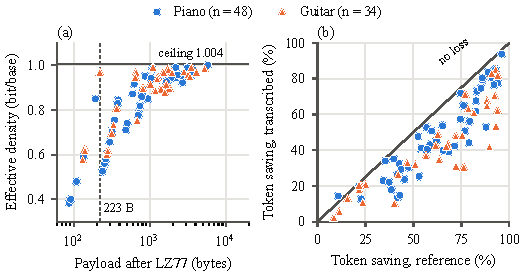
\includegraphics[width=\columnwidth]{fig3.pdf}
\caption{(a) Effective density against payload size after repeat detection. The dashed line marks one Reed--Solomon codeword (223 data bytes) and the solid line the ceiling of (\ref{eq:ceiling}). (b) Share of tokens removed by repeat detection on the reference notation and on the transcribed notes of each sample; points below the diagonal lost repetition to transcription errors.}
\label{fig:results}
\end{figure}

\subsection{Transcription Errors Reduce Exploitable Repetition}

Transcription errors cost compression as well as accuracy. On the reference notation, repeat detection removes 62.1\% of the tokens; on the transcribed notes of the same pieces it removes 45.7\%. The paired loss of $16.4 \pm 10.9$ percentage points occurs in 81 of the 82 samples (Wilcoxon $p < 10^{-14}$), as the points below the diagonal in Fig.~\ref{fig:results}(b) show. Spurious and displaced notes break phrases that are identical in the score, so about a quarter of the repetition in the music is lost before tokenisation. The ranking of pieces by repetitiveness is nevertheless preserved (Spearman $\rho = 0.91$), so repetitive music still compresses best.

\subsection{Reconstruction Accuracy}

The note-level F-measure averaged $0.748 \pm 0.152$ (Table~\ref{tab:results}). Recall (0.842) exceeded precision (0.692), so the dominant error is spurious notes rather than missed ones. Piano stems were transcribed far more accurately than guitar stems (0.806 against 0.666, Mann--Whitney $p < 0.001$), almost entirely through recall (0.918 against 0.736, $p < 0.001$). The measured content does not explain this gap. Piano and guitar stems do not differ significantly in polyphony, note density, chord share or spectral centroid ($p > 0.13$). The association of accuracy with the 14 signal and content properties was analysed as an exploratory question, with the false discovery rate controlled within each outcome by the Benjamini--Hochberg procedure \cite{bh}. No property was associated with the F-measure ($|\rho| \le 0.21$, $q \ge 0.42$). Precision was lower for pieces with longer notes ($\rho = -0.33$, $q = 0.031$) and higher for pieces with more attacks per second ($\rho = 0.30$, $q = 0.040$), and recall was lower for denser pieces, for pieces lying further from their grid and for pieces with a wider spread of velocities ($\rho$ from $-0.29$ to $-0.32$, $q = 0.041$). None of these survives correction across all 42 tests ($q \ge 0.064$), so they indicate where errors arise rather than confirm a hypothesis. The gap therefore most likely reflects the model's weaker handling of guitar timbres rather than the music played on them. The offset-aware F-measure was much lower for both instruments (0.292), in line with the known difficulty of detecting note endings \cite{benetos}.

The per-module scores locate the loss. Transcription reached $0.761 \pm 0.145$ against the reference, and the DNA stage was lossless. After quantisation about 9\% of the transcribed notes no longer matched their unquantised counterparts within tolerance (F-measure 0.909 against the transcription), yet the whole-system F-measure of 0.748 did not differ significantly from that of transcription alone (Wilcoxon $p = 0.67$, median difference zero; 36 samples improved, 28 degraded and 18 were unchanged): the gains and losses from rounding to the grid largely cancel. Improving the codec's accuracy therefore depends chiefly on the transcription model.

\subsection{Comparison with Published Schemes}

Table~\ref{tab:density} compares densities with published schemes, distinguishing the coding potential of the mapping alone from the net density after indexing, error correction and primers. The coding potential here, 1.58 bits per base, is that of the rotating code and is lower than that of more recent codes; this is the price of meeting the homopolymer constraint by construction. The net density is nevertheless competitive, although the comparison is indicative rather than a direct benchmark: the schemes differ in redundancy, indexing, primer design and channel assumptions, and the published figures come from synthesised and sequenced DNA whereas this work simulates the channel. The mean of 0.839 exceeds the 0.33 that Goldman et al. obtained with the same inner code and fourfold redundancy, and the longest samples approach the 1.14 of Grass et al., because the fixed overhead of primers, index and parity is modest and the padding of the final codeword is amortised over a long payload. The comparison concerns the DNA layer only, which is content-agnostic in every scheme listed; the token representation operates before it and could be combined with any of the denser inner codes.

\begin{table}[htbp]
\caption{Density Compared with Published Schemes (bits per base)}
\label{tab:density}
\centering
\footnotesize
\begin{tabular}{lcc}
\hline
\textbf{Scheme} & \textbf{Coding potential} & \textbf{Net density} \\
\hline
Church et al. \cite{church} & 1.00 & 0.83 \\
Goldman et al. \cite{goldman} & 1.58 & 0.33 \\
Grass et al. \cite{grass} & 1.78 & 1.14 \\
DNA Fountain \cite{erlich} & 1.98 & 1.57 \\
Yin--Yang codec \cite{ping} & 2.00 & not reported \\
DNA-Aeon \cite{welzel} & tunable & tunable \\
This work: mean (best) & 1.58 & 0.839 (1.000) \\
\hline
\multicolumn{3}{l}{Church, Goldman, Grass and DNA Fountain values as} \\
\multicolumn{3}{l}{tabulated in \cite{erlich}; Yin--Yang as reported in \cite{ping}; DNA-Aeon} \\
\multicolumn{3}{l}{sets its code rate per application \cite{welzel}.} \\
\end{tabular}
\end{table}

\subsection{Limitations}

The corpus contains only piano and guitar stems synthesised from MIDI; wind and bowed instruments, voice, ensemble mixtures and acoustic recordings are absent, and the large gap between the two instruments shows that the results depend on timbre. Excluding 56 tracks with tempo maps and 5 poorly fitting ones biases the corpus towards metrically regular music, as the small grid deviation in Table~\ref{tab:dataset} reflects, and samples cut from the same track are not fully independent. The DNA channel was simulated without errors, so the lossless round trip verifies the codec rather than its robustness; the design corrects substitutions through the Reed--Solomon code but not insertions or deletions, which desynchronise the rotating code \cite{press}, \cite{welzel}. Finally, the token scheme stores only pitch, onset and duration, so velocity, articulation and timbre are not preserved: the codec archives the notation of a recording, not its sound.

\section{Conclusion}

This paper presented a codec that stores music in DNA through its notation rather than the bytes of its audio, combining automatic transcription, a compact token scheme with token-level repeat detection, and a constraint-compliant encoding based on a Reed--Solomon outer code and a rotating inner code. On 82 quantitatively characterised piano and guitar stems it was lossless at the DNA layer, met all biochemical constraints, required 85.0\% fewer bases than the transcribed MIDI files and reached a note-level F-measure of 0.748; reconstruction error was dominated by transcription, and quantisation had no significant effect on the whole-system F-measure. The saving from repeat detection is limited by two effects measured here: codeword granularity, which hides it on short payloads, and transcription errors, which remove a quarter of the repetition in the music. Future work will extend the corpus to further instruments and to real recordings, support tempo changes, adopt a shortened Reed--Solomon code and a wider oligonucleotide index, add insertion and deletion correction, and pair the token representation with a denser inner code.

\section*{Acknowledgment}

The authors thank Universitas Pelita Harapan and its Institute of Research and Community Services (LPPM) for supporting this research under research number P-021-PDP-FTI/VII/2025.

\begin{thebibliography}{00}

\bibitem{dong} Y. Dong, F. Sun, Z. Ping, Q. Ouyang, and L. Qian, ``DNA storage: research landscape and future prospects,'' Natl. Sci. Rev., vol. 7, no. 6, pp. 1092--1107, Jun. 2020, doi: 10.1093/nsr/nwaa007.

\bibitem{lto} LTO Program, ``The benefits of LTO Ultrium tape technology,'' Linear Tape-Open Consortium. [Online]. Available: https://www.lto.org/benefits-of-lto/ (accessed Sep. 20, 2026).

\bibitem{shomorony} I. Shomorony and R. Heckel, ``Information-Theoretic Foundations of DNA Data Storage,'' Foundations and Trends in Communications and Information Theory, vol. 19, no. 1, pp. 1--106, Feb. 2022, doi: 10.1561/0100000117.

\bibitem{erlich} Y. Erlich and D. Zielinski, ``DNA Fountain enables a robust and efficient storage architecture,'' Science, vol. 355, no. 6328, pp. 950--954, Mar. 2017, doi: 10.1126/science.aaj2038.

\bibitem{grass} R. N. Grass, R. Heckel, M. Puddu, D. Paunescu, and W. J. Stark, ``Robust chemical preservation of digital information on DNA in silica with error-correcting codes,'' Angew. Chem. Int. Ed., vol. 54, no. 8, pp. 2552--2555, Feb. 2015, doi: 10.1002/anie.201411378.

\bibitem{dufaux} A. Dufaux and T. Amsallem, ``The Montreux Jazz Digital Project: From preserving heritage to a platform for innovation,'' J. Digit. Media Manag., vol. 7, no. 4, p. 315, Jun. 2019, doi: 10.69554/HKXL1171.

\bibitem{lee} H. Lee et al., ``Photon-directed multiplexed enzymatic DNA synthesis for molecular digital data storage,'' Nat. Commun., vol. 11, no. 1, p. 5246, Oct. 2020, doi: 10.1038/s41467-020-18681-5.

\bibitem{yu} M. Yu et al., ``High-throughput DNA synthesis for data storage,'' Chem. Soc. Rev., vol. 53, no. 9, pp. 4463--4489, 2024, doi: 10.1039/D3CS00469D.

\bibitem{benetos} E. Benetos, S. Dixon, Z. Duan, and S. Ewert, ``Automatic Music Transcription: An Overview,'' IEEE Signal Process. Mag., vol. 36, no. 1, pp. 20--30, Jan. 2019, doi: 10.1109/MSP.2018.2869928.

\bibitem{church} G. M. Church, Y. Gao, and S. Kosuri, ``Next-generation digital information storage in DNA,'' Science, vol. 337, no. 6102, p. 1628, Sep. 2012, doi: 10.1126/science.1226355.

\bibitem{goldman} N. Goldman et al., ``Towards practical, high-capacity, low-maintenance information storage in synthesized DNA,'' Nature, vol. 494, no. 7435, pp. 77--80, Feb. 2013, doi: 10.1038/nature11875.

\bibitem{schwarz} P. M. Schwarz and B. Freisleben, ``Data recovery methods for DNA storage based on fountain codes,'' Comput. Struct. Biotechnol. J., vol. 23, pp. 1808--1823, Dec. 2024, doi: 10.1016/j.csbj.2024.04.048.

\bibitem{organick} L. Organick et al., ``Random access in large-scale DNA data storage,'' Nat. Biotechnol., vol. 36, no. 3, pp. 242--248, Mar. 2018, doi: 10.1038/nbt.4079.

\bibitem{lochel} H. F. L\"ochel, M. Welzel, G. Hattab, A.-C. Hauschild, and D. Heider, ``Fractal construction of constrained code words for DNA storage systems,'' Nucleic Acids Res., vol. 50, no. 5, pp. e30--e30, Mar. 2022, doi: 10.1093/nar/gkab1209.

\bibitem{ping} Z. Ping et al., ``Towards practical and robust DNA-based data archiving using the yin--yang codec system,'' Nat. Comput. Sci., vol. 2, no. 4, pp. 234--242, Apr. 2022, doi: 10.1038/s43588-022-00231-2.

\bibitem{cao} B. Cao, X. Zhang, S. Cui, and Q. Zhang, ``Adaptive coding for DNA storage with high storage density and low coverage,'' NPJ Syst. Biol. Appl., vol. 8, no. 1, p. 23, Jul. 2022, doi: 10.1038/s41540-022-00233-w.

\bibitem{welzel} M. Welzel et al., ``DNA-Aeon provides flexible arithmetic coding for constraint adherence and error correction in DNA storage,'' Nat. Commun., vol. 14, no. 1, p. 628, Feb. 2023, doi: 10.1038/s41467-023-36297-3.

\bibitem{press} W. H. Press, J. A. Hawkins, S. K. Jones Jr., J. M. Schaub, and I. J. Finkelstein, ``HEDGES error-correcting code for DNA storage corrects indels and allows sequence constraints,'' Proc. Natl. Acad. Sci. U.S.A., vol. 117, no. 31, pp. 18489--18496, Aug. 2020, doi: 10.1073/pnas.2004821117.

\bibitem{preuss} I. Preuss, M. Rosenberg, Z. Yakhini, and L. Anavy, ``Efficient DNA-based data storage using shortmer combinatorial encoding,'' Sci. Rep., vol. 14, no. 1, p. 7731, Apr. 2024, doi: 10.1038/s41598-024-58386-z.

\bibitem{xu} C. Xu, C. Zhao, B. Ma, and H. Liu, ``Uncertainties in synthetic DNA-based data storage,'' Nucleic Acids Res., vol. 49, no. 10, pp. 5451--5469, Jun. 2021, doi: 10.1093/nar/gkab230.

\bibitem{bittner} R. M. Bittner, J. J. Bosch, D. Rubinstein, G. Meseguer-Brocal, and S. Ewert, ``A Lightweight Instrument-Agnostic Model for Polyphonic Note Transcription and Multipitch Estimation,'' in ICASSP 2022 -- 2022 IEEE International Conference on Acoustics, Speech and Signal Processing (ICASSP), Singapore, May 2022, pp. 781--785, doi: 10.1109/ICASSP43922.2022.9746549.

\bibitem{antkowiak} P. L. Antkowiak et al., ``Low cost DNA data storage using photolithographic synthesis and advanced information reconstruction and error correction,'' Nat. Commun., vol. 11, no. 1, p. 5345, Oct. 2020, doi: 10.1038/s41467-020-19148-3.

\bibitem{kiryanova} O. Y. Kiryanova, R. R. Garafutdinov, I. M. Gubaydullin, and A. V. Chemeris, ``A novel approach to encode melodies in DNA,'' BioSystems, vol. 237, p. 105136, Mar. 2024, doi: 10.1016/j.biosystems.2024.105136.

\bibitem{ziv} J. Ziv and A. Lempel, ``A universal algorithm for sequential data compression,'' IEEE Trans. Inf. Theory, vol. 23, no. 3, pp. 337--343, May 1977, doi: 10.1109/TIT.1977.1055714.

\bibitem{reed} I. S. Reed and G. Solomon, ``Polynomial Codes Over Certain Finite Fields,'' Journal of the Society for Industrial and Applied Mathematics, vol. 8, no. 2, pp. 300--304, Jun. 1960, doi: 10.1137/0108018.

\bibitem{slakh} E. Manilow, G. Wichern, P. Seetharaman, and J. Le Roux, ``Cutting music source separation some Slakh: A dataset to study the impact of data quality on source separation performance,'' in 2019 IEEE Workshop on Applications of Signal Processing to Audio and Acoustics (WASPAA), New Paltz, NY, USA, Oct. 2019, pp. 45--49, doi: 10.1109/WASPAA.2019.8937170.

\bibitem{raffel} C. Raffel et al., ``mir\_eval: A transparent implementation of common MIR metrics,'' in Proc. 15th Int. Soc. Music Information Retrieval Conf. (ISMIR), Taipei, Taiwan, Oct. 2014, pp. 367--372.

\bibitem{bh} Y. Benjamini and Y. Hochberg, ``Controlling the false discovery rate: A practical and powerful approach to multiple testing,'' J. R. Stat. Soc. Ser. B (Methodol.), vol. 57, no. 1, pp. 289--300, 1995, doi: 10.1111/j.2517-6161.1995.tb02031.x.

\end{thebibliography}

\end{document}
